% Options for packages loaded elsewhere
\PassOptionsToPackage{unicode}{hyperref}
\PassOptionsToPackage{hyphens}{url}
%
\documentclass[
]{article}
\usepackage{amsmath,amssymb}
\usepackage{lmodern}
\usepackage{iftex}
\ifPDFTeX
  \usepackage[T1]{fontenc}
  \usepackage[utf8]{inputenc}
  \usepackage{textcomp} % provide euro and other symbols
\else % if luatex or xetex
  \usepackage{unicode-math}
  \defaultfontfeatures{Scale=MatchLowercase}
  \defaultfontfeatures[\rmfamily]{Ligatures=TeX,Scale=1}
\fi
% Use upquote if available, for straight quotes in verbatim environments
\IfFileExists{upquote.sty}{\usepackage{upquote}}{}
\IfFileExists{microtype.sty}{% use microtype if available
  \usepackage[]{microtype}
  \UseMicrotypeSet[protrusion]{basicmath} % disable protrusion for tt fonts
}{}
\makeatletter
\@ifundefined{KOMAClassName}{% if non-KOMA class
  \IfFileExists{parskip.sty}{%
    \usepackage{parskip}
  }{% else
    \setlength{\parindent}{0pt}
    \setlength{\parskip}{6pt plus 2pt minus 1pt}}
}{% if KOMA class
  \KOMAoptions{parskip=half}}
\makeatother
\usepackage{xcolor}
\usepackage[margin=1in]{geometry}
\usepackage{color}
\usepackage{fancyvrb}
\newcommand{\VerbBar}{|}
\newcommand{\VERB}{\Verb[commandchars=\\\{\}]}
\DefineVerbatimEnvironment{Highlighting}{Verbatim}{commandchars=\\\{\}}
% Add ',fontsize=\small' for more characters per line
\usepackage{framed}
\definecolor{shadecolor}{RGB}{248,248,248}
\newenvironment{Shaded}{\begin{snugshade}}{\end{snugshade}}
\newcommand{\AlertTok}[1]{\textcolor[rgb]{0.94,0.16,0.16}{#1}}
\newcommand{\AnnotationTok}[1]{\textcolor[rgb]{0.56,0.35,0.01}{\textbf{\textit{#1}}}}
\newcommand{\AttributeTok}[1]{\textcolor[rgb]{0.77,0.63,0.00}{#1}}
\newcommand{\BaseNTok}[1]{\textcolor[rgb]{0.00,0.00,0.81}{#1}}
\newcommand{\BuiltInTok}[1]{#1}
\newcommand{\CharTok}[1]{\textcolor[rgb]{0.31,0.60,0.02}{#1}}
\newcommand{\CommentTok}[1]{\textcolor[rgb]{0.56,0.35,0.01}{\textit{#1}}}
\newcommand{\CommentVarTok}[1]{\textcolor[rgb]{0.56,0.35,0.01}{\textbf{\textit{#1}}}}
\newcommand{\ConstantTok}[1]{\textcolor[rgb]{0.00,0.00,0.00}{#1}}
\newcommand{\ControlFlowTok}[1]{\textcolor[rgb]{0.13,0.29,0.53}{\textbf{#1}}}
\newcommand{\DataTypeTok}[1]{\textcolor[rgb]{0.13,0.29,0.53}{#1}}
\newcommand{\DecValTok}[1]{\textcolor[rgb]{0.00,0.00,0.81}{#1}}
\newcommand{\DocumentationTok}[1]{\textcolor[rgb]{0.56,0.35,0.01}{\textbf{\textit{#1}}}}
\newcommand{\ErrorTok}[1]{\textcolor[rgb]{0.64,0.00,0.00}{\textbf{#1}}}
\newcommand{\ExtensionTok}[1]{#1}
\newcommand{\FloatTok}[1]{\textcolor[rgb]{0.00,0.00,0.81}{#1}}
\newcommand{\FunctionTok}[1]{\textcolor[rgb]{0.00,0.00,0.00}{#1}}
\newcommand{\ImportTok}[1]{#1}
\newcommand{\InformationTok}[1]{\textcolor[rgb]{0.56,0.35,0.01}{\textbf{\textit{#1}}}}
\newcommand{\KeywordTok}[1]{\textcolor[rgb]{0.13,0.29,0.53}{\textbf{#1}}}
\newcommand{\NormalTok}[1]{#1}
\newcommand{\OperatorTok}[1]{\textcolor[rgb]{0.81,0.36,0.00}{\textbf{#1}}}
\newcommand{\OtherTok}[1]{\textcolor[rgb]{0.56,0.35,0.01}{#1}}
\newcommand{\PreprocessorTok}[1]{\textcolor[rgb]{0.56,0.35,0.01}{\textit{#1}}}
\newcommand{\RegionMarkerTok}[1]{#1}
\newcommand{\SpecialCharTok}[1]{\textcolor[rgb]{0.00,0.00,0.00}{#1}}
\newcommand{\SpecialStringTok}[1]{\textcolor[rgb]{0.31,0.60,0.02}{#1}}
\newcommand{\StringTok}[1]{\textcolor[rgb]{0.31,0.60,0.02}{#1}}
\newcommand{\VariableTok}[1]{\textcolor[rgb]{0.00,0.00,0.00}{#1}}
\newcommand{\VerbatimStringTok}[1]{\textcolor[rgb]{0.31,0.60,0.02}{#1}}
\newcommand{\WarningTok}[1]{\textcolor[rgb]{0.56,0.35,0.01}{\textbf{\textit{#1}}}}
\usepackage{graphicx}
\makeatletter
\def\maxwidth{\ifdim\Gin@nat@width>\linewidth\linewidth\else\Gin@nat@width\fi}
\def\maxheight{\ifdim\Gin@nat@height>\textheight\textheight\else\Gin@nat@height\fi}
\makeatother
% Scale images if necessary, so that they will not overflow the page
% margins by default, and it is still possible to overwrite the defaults
% using explicit options in \includegraphics[width, height, ...]{}
\setkeys{Gin}{width=\maxwidth,height=\maxheight,keepaspectratio}
% Set default figure placement to htbp
\makeatletter
\def\fps@figure{htbp}
\makeatother
\setlength{\emergencystretch}{3em} % prevent overfull lines
\providecommand{\tightlist}{%
  \setlength{\itemsep}{0pt}\setlength{\parskip}{0pt}}
\setcounter{secnumdepth}{-\maxdimen} % remove section numbering
\ifLuaTeX
  \usepackage{selnolig}  % disable illegal ligatures
\fi
\IfFileExists{bookmark.sty}{\usepackage{bookmark}}{\usepackage{hyperref}}
\IfFileExists{xurl.sty}{\usepackage{xurl}}{} % add URL line breaks if available
\urlstyle{same} % disable monospaced font for URLs
\hypersetup{
  pdftitle={Ejemplo Integración Monte Carlo},
  pdfauthor={Guillermo Durán González},
  hidelinks,
  pdfcreator={LaTeX via pandoc}}

\title{Ejemplo Integración Monte Carlo}
\author{Guillermo Durán González}
\date{2022-11-05}

\begin{document}
\maketitle

\hypertarget{ejemplo-de-integraciuxf3n-monte-carlo}{%
\section{Ejemplo de Integración Monte
Carlo}\label{ejemplo-de-integraciuxf3n-monte-carlo}}

\hypertarget{estimemos-el-valor-de-la-siguiente-integral-usando-monte-carlo}{%
\subsection{Estimemos el valor de la siguiente integral usando Monte
Carlo:}\label{estimemos-el-valor-de-la-siguiente-integral-usando-monte-carlo}}

\[
\theta=\int_0^1 e^{-x} d x
\] \# Apliquemos el siguiente script:

\begin{Shaded}
\begin{Highlighting}[]
\NormalTok{n }\OtherTok{\textless{}{-}} \DecValTok{10000}
\NormalTok{x }\OtherTok{\textless{}{-}} \FunctionTok{runif}\NormalTok{(n)}
\NormalTok{media}\OtherTok{\textless{}{-}}\FunctionTok{mean}\NormalTok{(}\FunctionTok{exp}\NormalTok{(}\SpecialCharTok{{-}}\NormalTok{x))}
\NormalTok{theta }\OtherTok{\textless{}{-}}\NormalTok{ media}\SpecialCharTok{*}\NormalTok{(}\DecValTok{1{-}0}\NormalTok{)}
\FunctionTok{print}\NormalTok{(theta)}
\end{Highlighting}
\end{Shaded}

\begin{verbatim}
## [1] 0.6345205
\end{verbatim}

\hypertarget{en-la-gruxe1fica-se-puede-notar-en-rojo-la-media}{%
\subsection{En la gráfica se puede notar en rojo la
media:}\label{en-la-gruxe1fica-se-puede-notar-en-rojo-la-media}}

\begin{Shaded}
\begin{Highlighting}[]
\FunctionTok{plot}\NormalTok{(x, }\FunctionTok{exp}\NormalTok{(}\SpecialCharTok{{-}}\NormalTok{x),}\AttributeTok{xlab=}\StringTok{"x"}\NormalTok{, }\AttributeTok{ylab=}\StringTok{"e\^{}({-}x)"}\NormalTok{, }\AttributeTok{type=}\StringTok{"p"}\NormalTok{,}\AttributeTok{col=}\StringTok{"green"}\NormalTok{, }\AttributeTok{xlim=}\FunctionTok{c}\NormalTok{(}\DecValTok{0}\NormalTok{,}\DecValTok{1}\NormalTok{))}
\FunctionTok{text}\NormalTok{(}\FloatTok{0.5}\NormalTok{,media}\FloatTok{{-}0.025}\NormalTok{, }\StringTok{"Media"}\NormalTok{, }\AttributeTok{col=}\StringTok{"red"}\NormalTok{) }
\FunctionTok{abline}\NormalTok{(}\AttributeTok{h=}\NormalTok{media, }\AttributeTok{col=}\StringTok{"red"}\NormalTok{)}
\end{Highlighting}
\end{Shaded}

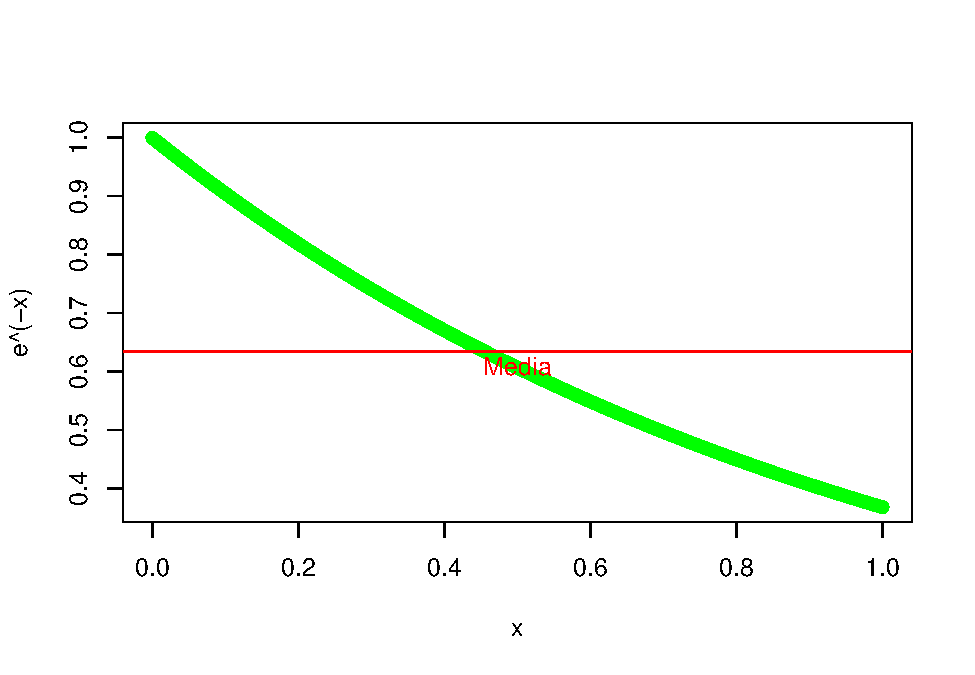
\includegraphics{Ejemplo-Integración-Monte-Carlo_files/figure-latex/remedy003-1.pdf}

\hypertarget{notese-que-al-resolver-la-integral-obtenemos-un-valor-similar}{%
\subsection{Notese que al resolver la integral obtenemos un valor
similar:}\label{notese-que-al-resolver-la-integral-obtenemos-un-valor-similar}}

\[
\int_0^1 e^{-x} d x=-e^{-x}\Big|_0^1=1-\frac{1}{e}= 0.6321206
\]

\newpage

\hypertarget{obtenga-el-valor-de-la-siguiente-integral-usando-monte-carlo}{%
\subsection{Obtenga el valor de la siguiente integral usando Monte
Carlo:}\label{obtenga-el-valor-de-la-siguiente-integral-usando-monte-carlo}}

\[
\theta=\int_2^4 e^{-x} d x
\] Solución: Mediante Monte Carlo se encuentra el siguiente valor:

\begin{Shaded}
\begin{Highlighting}[]
\NormalTok{n }\OtherTok{\textless{}{-}} \DecValTok{10000}
\NormalTok{x }\OtherTok{\textless{}{-}} \FunctionTok{runif}\NormalTok{(n, }\AttributeTok{min=}\DecValTok{2}\NormalTok{, }\AttributeTok{max=}\DecValTok{4}\NormalTok{ )}
\NormalTok{media}\OtherTok{\textless{}{-}}\FunctionTok{mean}\NormalTok{(}\FunctionTok{exp}\NormalTok{(}\SpecialCharTok{{-}}\NormalTok{x))}
\NormalTok{theta }\OtherTok{\textless{}{-}}\NormalTok{ media}\SpecialCharTok{*}\NormalTok{(}\DecValTok{4{-}2}\NormalTok{)}
\FunctionTok{plot}\NormalTok{(x, }\FunctionTok{exp}\NormalTok{(}\SpecialCharTok{{-}}\NormalTok{x),}\AttributeTok{xlab=}\StringTok{"x"}\NormalTok{, }\AttributeTok{ylab=}\StringTok{"e\^{}({-}x)"}\NormalTok{,}\AttributeTok{col=}\StringTok{"green"}\NormalTok{, }
     \AttributeTok{xlim=}\FunctionTok{c}\NormalTok{(}\DecValTok{2}\NormalTok{,}\DecValTok{4}\NormalTok{), }\AttributeTok{ylim=}\FunctionTok{c}\NormalTok{(}\DecValTok{0}\NormalTok{,theta}\FloatTok{+.1}\NormalTok{),}\AttributeTok{type=}\StringTok{"p"}\NormalTok{)}
\FunctionTok{text}\NormalTok{(}\DecValTok{3}\NormalTok{,media}\FloatTok{+0.05}\NormalTok{, }\StringTok{"Media"}\NormalTok{, }\AttributeTok{col=}\StringTok{"red"}\NormalTok{)}
\FunctionTok{abline}\NormalTok{(}\AttributeTok{h=}\NormalTok{media, }\AttributeTok{col=}\StringTok{"red"}\NormalTok{)}
\end{Highlighting}
\end{Shaded}

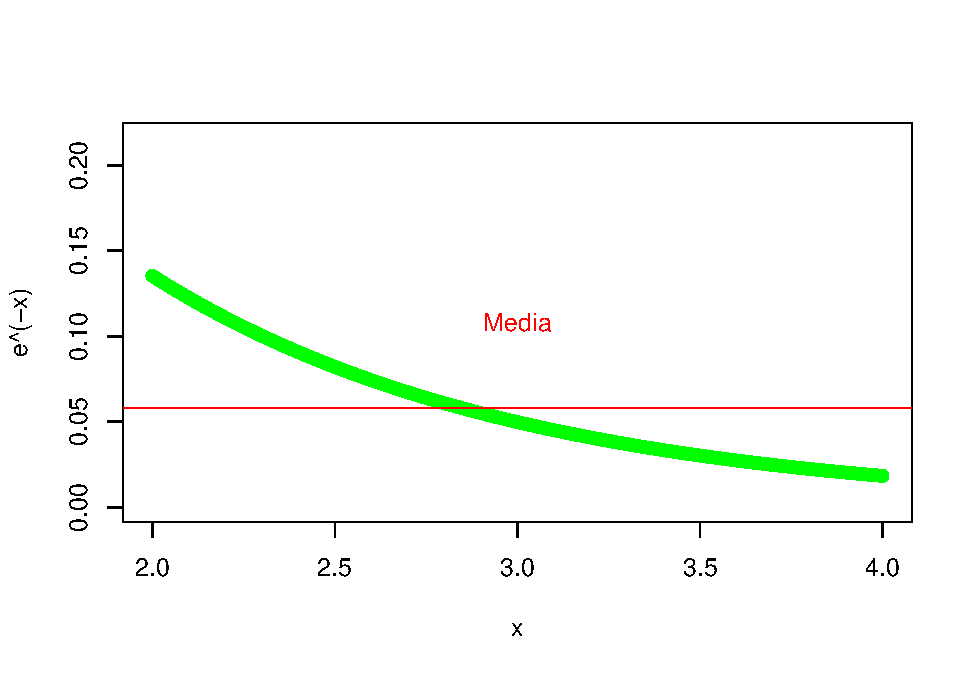
\includegraphics{Ejemplo-Integración-Monte-Carlo_files/figure-latex/remedy002-1.pdf}

\begin{Shaded}
\begin{Highlighting}[]
\FunctionTok{print}\NormalTok{(theta)}
\end{Highlighting}
\end{Shaded}

\begin{verbatim}
## [1] 0.1160732
\end{verbatim}

\hypertarget{resolviendo-la-integral-se-obtiene}{%
\section{Resolviendo la integral se
obtiene:}\label{resolviendo-la-integral-se-obtiene}}

\[
\int_2^4 e^{-x} d x=-e^{-x}\Big|_2^4=\frac{1}{e^2}-\frac{1}{e^4}= 0.11701...
\]

\end{document}
